\subsection{Testing for Credentials Transported over an Encrypted Channel - OTG-AUTHN-001} \label{OTG-AUTHN-001}

\paragraph{BANK-APP} \mbox{}
\begin{longtable*}{p{.20\textwidth} | p{.80\textwidth}}
    \hline
    & \textbf{BANK-APP} \\
    \hline
    \textbf{Observation} &
     After scanning the application with the Vega tool, it was found that the forms in the Registration, Login and Create Transaction pages submit to an insecure HTTP target. Parameters such as User name, Password, TAN number, Account ID are not encrypted. 
    \\\\
    \textbf{Discovery} &
       Three tools Vega, Burp Suite and cURL were used to discover this vulnerability.Steps are as follows:
       \begin{itemize}
       	\item \underline{\textbf{Vega}}
       		\begin{itemize}
       			\item Click on the Scan tab and enter the URL to be tested. In our case, it was "\textit{http://<IP-address>/secure-coding/public/login.php}".
       			
       			\item Click on the Finish button. A report is generated which has three sections - High, Low, Info. This vulnerability is termed as "Clear Password over HTTP" and falls under the High section. See Figure \ref{fig:password_over_http}
       		\end{itemize}
       	\item After detection, one more tool-the Burp Suite was used to delve deeper into it.\underline{\textbf{Burp Suite}}
       		\begin{itemize}
       			\item Open Burp Suite Tool. Click on Proxy tab and set interception to on. This will enable us to observe all the requests to be monitored before being served.
       			
       		  \item Now open the browser and under tools, set Foxy Proxy standard to use Burp Suite for all URLs .
       		  
       		  \item On the Login page, enter the details and click on Submit.
       		  
       		  \item Now click  on the Proxy tab in the Burp Suite. The requested URL data which contains Username and password can be seen in the Raw tab as plain text; revealing that the request was not encrypted. This could be used by the attacker to impersonate as the victim. 
       		\end{itemize}
       	\item To verify whether the application works on HTTP or HTTPS, cURL was used. \underline{\textbf{cURL}}
       		\begin{itemize}
       		  \item Open the terminal and type curl https://<IP-address>.
       		         The response states unknown protocol. 
       		 \item  To get a detailed response, use curl --verbose https://<IP-address>.
       		 
       		 \item Now try with curl http://<IP-address>.
       		        The response indicates a successful connection and the output of the request. See Figure \ref{fig:curl_https}.
       		        It can be concluded that the application works only on HTTP and does not support transmission over HTTPS.
       		\end{itemize}
       \end{itemize} 
    \\\\
    \textbf{Likelihood} &
        Likelihood is high since this takes place over the network.
        Exploitation of this vulnerability requires basic knowledge of any monitoring tools to view the format and details of the server requests. It is exploitable remotely.
    \\\\
    \textbf{Impact} &
        A successful attack might lead to serious consequences. The request parameters can be tampered with, as they are not encrypted. This may lead to the victim not being able to login  or transactions being hijacked. This could result in a Denial of Service attack as well.
    \\\\
    \textbf{CVSS} &
      \begin{tabular}{| l | l |}
      \hline
      Attack Vector		& \textit{Network}\\
      \hline
      Attack Complexity	& \textit{Low} \\
      \hline
      Privileges Required & \textit{Low} \\
      \hline
      User Interaction	& \textit{None} \\
      \hline
      Scope		& \textit{Unchanged} \\
      \hline
      Confidentiality	& \textit{High} \\
      \hline
      Integrity		& \textit{High} \\
      \hline
      Availability		& \textit{High} \\
      \hline
      \end{tabular}
    \\
    \hline
\end{longtable*}

\begin{figure}[ht]
	\centering
		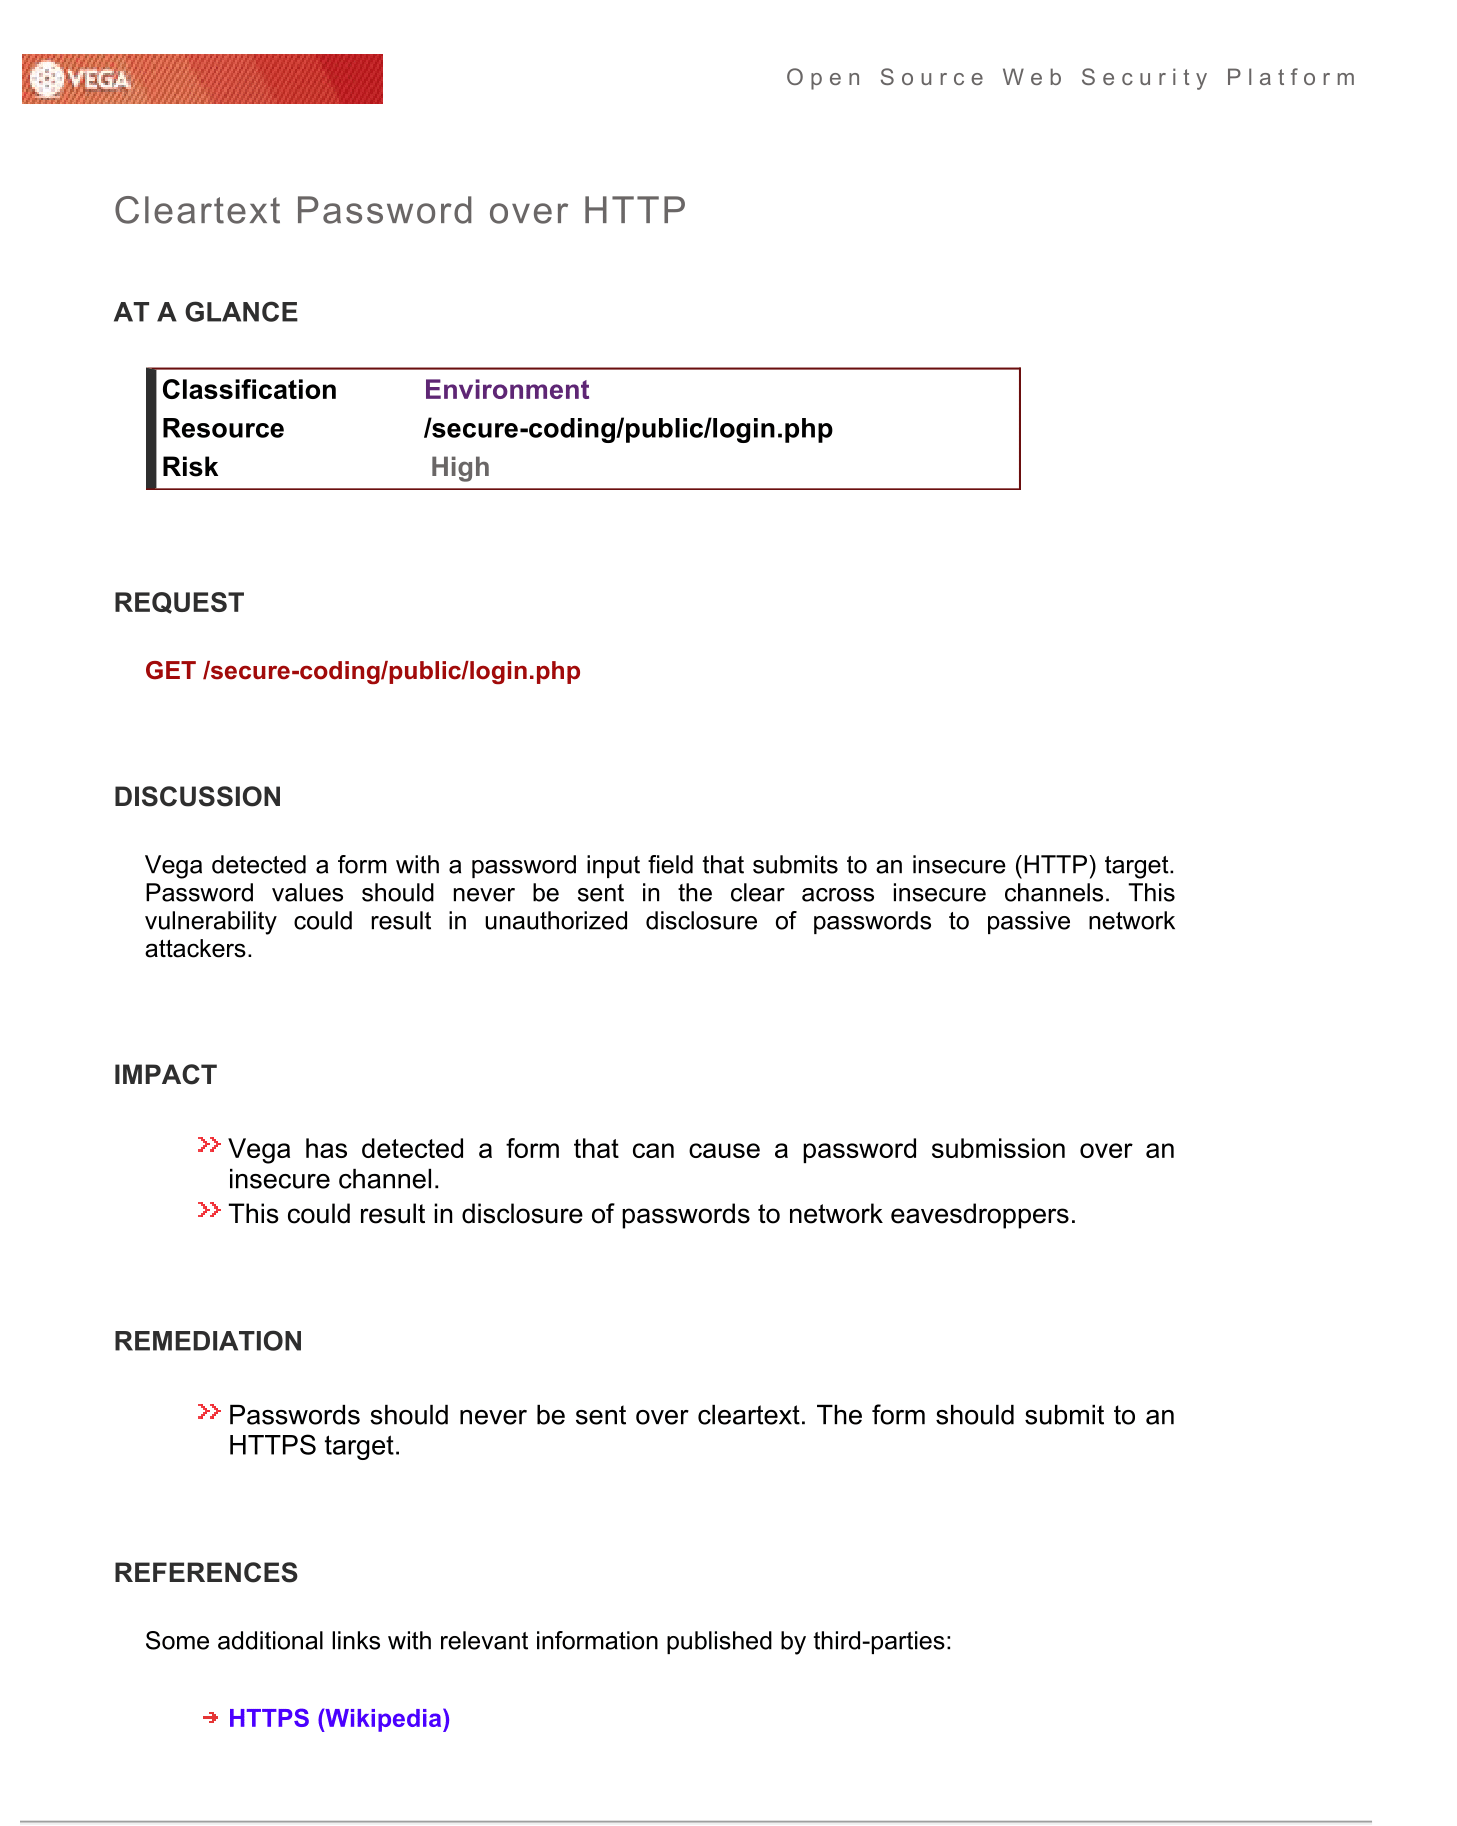
\includegraphics[width=.8\linewidth]{figures/OTG-AUTHN-001_1.png}
		\caption{Vega Report-Clear password over HTTP}
	\label{fig:password_over_http}
\end{figure}
\begin{figure}[ht]
	\centering
		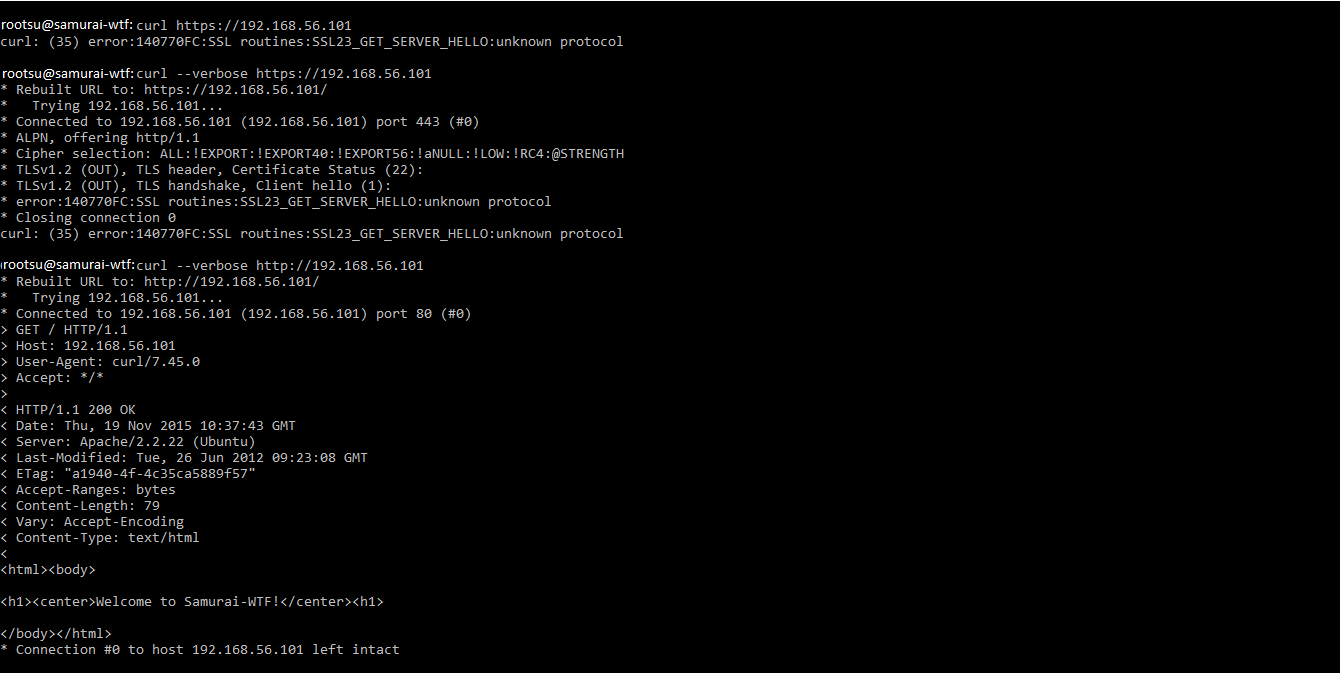
\includegraphics[width=.8\linewidth]{figures/OTG-AUTHN-001_2.png}
		\caption{cURL - Check for HTTPS}
	\label{fig:curl_https}
\end{figure}

\paragraph{SecureBank} \mbox{}
\begin{longtable*}{p{.20\textwidth} | p{.80\textwidth}}
    \hline
    & \textbf{SecureBank} \\
    \hline
    \textbf{Observation} &
       After scanning the application with the Vega tool, it was found that the forms in the Registration, Login and Create Transaction pages submit to an insecure HTTP target. Parameters such as User name, Password, TAN number, Account ID are not encrypted.
    \\\\
    \textbf{Discovery} &
    The same vulnerability exists in our application as well; since the channel over which the communication takes place is not encrypted.
    \\\\
    \textbf{Likelihood} &
        Same as described for BANK-APP.
    \\\\
    \textbf{Impact} &
        Same as described for BANK-APP.
    \\\\
    \textbf{CVSS} &
        Same as described for BANK-APP.
    \\
    \hline
\end{longtable*}
\clearpage